\documentclass[12pt, letterpaper]{article}
\usepackage{graphicx}
\usepackage{lastpage}

\begin{document}

\begin{titlepage}

\begin{center}

\includegraphics[width=.5\textwidth]{./bee}\\[2cm]
\textsc{\LARGE Project Plan For}\\[1.5cm]
\textsc{\LARGE Tellagence Capstone Project}\\[1.5cm]
\textsc{\LARGE Team Beeeeees}\\[1.5cm]
\large Team Members: Aren Edlund-Jermain, Jonathan Harker, Derek Hurley, Tien Le, Long Nguyen, Huy Tran\\
\hfill \\
\end{center}

\vfill

\end{titlepage}

\tableofcontents
\pagebreak 

\section{Overview}
	\subsection{Objective}
	The objective of this project is essentially to model and visualize the strengths of relationships on Twitter. This will be a web based application that renders a visual representation of the relationships between users on Twitter and the strengths of those relationships to show who are the most influential users in different networks of users.
  \subsection{Requirements}
	In talks with Matt and Nitin from Tellagence, we gathered and understood the following requirements:
	\begin{itemize}
		\item The relationships themselves are defined by interactions between users via `@' mentions and retweets.
		\item The mention and retweet values will be parsed from Twitter data into a database in a format for the rendering.
		\item The rendering needs to be usable and coherent, not just a tangled mess of nodes and connections.
		\item Directions of the relationships matters, meaning mentioning someone is one direction while retweeting them is the other.
        \item Directionality on the graph renderings will be shown by arrows as the links between users.
		\item Strengths of the relationships are determined by frequency of mentions/retweets between users over 7 days.
        \item Increased node degree (connectedness) will be shown by increased node size.
        \item The stronger the relationship between two users, the thicker and short their link.
		\item We need to be able to parse multiple `@' mentions out of a single tweet, and distinguish between `@' and `RT @'.
		\item The purpose of the visual is about predicting behavior and showing which users are the most influential, meaning the most meaningful connections.
        \item Users will have the ability to search by Twitter username to center the graph around the searched user.
        \item To model disjoint subgraphs, a separate visual showing all the subgraphs in a coherent form is needed with navigation between the two visuals.
        \item While rendering the visual, the user should have a progress bar let them know the status of the rendering.
        \item Making the visuals interactive is important, so zooming and panning across the graph is required.
	\end{itemize}

  \subsection{Approach}
	To complete this project, three main sections of the project have been identified: Data Handling, Rendering, and Interface. These three sections are planned to be completed in parallel, with milestones and tasks broken down in each. The plan is to speed up development by coding in parallel and doing a minimal implementations of the requirements first, then building on those implementations incrementally for a better finished product.
	\\\\
	The scheduled tasks and milestones should be contained to an eight week time frame. This allows for two weeks of spare time at the end of the term prior to the final deadline, which helps save us if and when issues arise concerning the project that merit more time than originally budgeted. With the milestones lining up as well, there should be a very basic iteration of the project by around the fourth week in the time line.

\section{Role Descriptions}
  \subsection{Aren Edlund-Jermain}
  {\bf Testing and Validation:} Must ensure that software passes tests and meets requirements. Check each stage of process to ensure proper software behavior with unit tests. Stay aware of client specifications and ensure that software project meets those goals. Maintain automatic build system. Write appropriate unit tests for each individual piece of project.
  \subsection{Derek Hurley}
  {\bf Team Lead and Sponsor Contact:} Team Lead must plan meetings, aid in overall design and implementation of the project, mediate conflicts between team members, and generally make sure work is completed in an efficient manner. Sponsor Contact must maintain frequent communication with the team sponsors to keep them aware of the project status and gather requirements/clarifications as needed.
  \subsection{Huy Tran}
  {\bf Documentation Lead:} Documentation Lead must ensure the following. First, having a agreed template for a document which is suitable for each team member to add their contents into it. Second, there are sufficient, up to date documents for all parts of the project. At the end of each development phase, Documentation Lead must ensure that all documents for all parts are integrated into one comprehensive document.
  \subsection{Jonathan Harker}
  {\bf Issues and Ticketing Lead:} Ensure that deadlines are met, bugs are resolved in a timely manner, and the project moves forward as planned.
  \subsection{Long Nguyen}
  {\bf Architectural Design and Tech Lead:} Prospect the scope of the entire project and construct architecture. Coordinate with all programmers to keep improving architectural design. Do major research on GUI tech and demo for other members.
  \subsection{Tien Le}
  {\bf System Administrator Lead:} Install, patch and upgrade servers. Keep all of the servers running 24/7. Build PHPUnit test.

\section{Arrange Nodes Approach}
 \subsection{Introduction}
  The purpose of arranging nodes is to visualize the relationship of
  users (nodes) in two directional Euclidean space by defining and using Euclidean distances between
  every nodes. There are two main benefits of arranging nodes. First,
  since a node is put into a graph by considering its relative
  position to all other nodes in the graph, it prevents the cases
  which a node is put randomly into the graph, so that the graph looks
  consistent everytime. Second, by tranforming the relationship between
  users into the Euclidean distances, the relationships between nodes
  can be recognized by observing the relative distance between them. 
 \subsection{Approach}
 The main idea of this approach is mapping the strength of
 relationship between nodes into Euclidean distance and displaying the
 Euclidean distances in two dimensional space. 
  \subsubsection{Mapping the strength of relationship into Euclidean distance}
First of all, we define the distance between two nodes as the inverse of
the strength of relationship which are the number of times which these
two nodes(users) talk together. It is reasonable because the stronger
the relationship between two nodes is, the smaller the distance between
them.
\\Second, based on these distances, we generate the Euclidean distances
between every nodes by following the properties of Euclidean
spaces. Euclidean (metric) space are introduced by Maurice Fréchet\footnote{Maurice Fréchet introduced metric spaces in his work Sur quelques points du calcul fonctionnel, Rendic. Circ. Mat. Palermo 22 (1906) 1–74.}. Let
a metric space be an ordered pair (M,d) where M is a set and d is
metric on M,i.e., a function d: M x M $\rightarrow$ R such that for any x,y,z 
$\in$ M, the following holds: 
 \begin{itemize}
    \item d(x,y) $\geq$ 0 
    \item d(x,y) = 0 iff x = y
    \item d(x,y) = d(y,x)
    \item d(x,z) $\leq$ d(x,y) + d(y,z)
  \end{itemize}
The mapping is defined as the distance between any two nodes is the
shortest distance between them. By the definition of this
mapping, it is clear to see that the distances between any two nodes
satisfy the first three properties of Euclidean space. There is a
proof for it also follows the last properties.
  \begin{itemize}
    \item For any nodes x, y, and z, we need to prove d(x,y)  $\leq$
      d(x,z) + d(z,y) with d(x,y), d(x,z), and d(z,y) are the shortest
      distance between these pair of nodes.
    \item Assume that d(x,y) > d(x,z) + d(z,y) then it is clear
      that d(x,y) is not the shortest distance from x to
      y. (Contrapositive proof)
  \end{itemize}
  \subsubsection{Displaying Euclidean distance in two dimensional space}
   After mapping the strength of relationship into Euclidean distance,
   this part shows how we display Euclidean distance in two dimensional
   space. Since it is impossible to display all of Euclidean distances
   in two dimensional space, there are two ways for dealing with this
   problem.
     \begin{itemize}
       \item Euclidean distances are approximated in two dimensional
         space.  Approximation is provided by d3 framework by allowing
         simple contrainsts\footnote{Tim Dwyer. Scalable, versatile and simple constrained graph layout. In Proc. Eurographics/IEEE-VGTC Symp. on Visualization (Eurovis 2009). (to appear) IEEE, 2009.}.
       \item The relationship is also indicated by other signal like
         the width of links between two nodes.
     \end{itemize}

 \subsection{Conclusion}
   \begin{itemize}
       \item Applying this approach in d3's force framework allows
         rendering thousands of nodes. 
       \item For most of the links, we can still see the relation between the width of the link
         and the distance between two nodes in the graph consisting
         of thousands of nodes. Also, due to the requirements and the
         scope of this project, we have not calculate the percentage
         of correctness of this approach.
     \end{itemize}

\section{Task Schedule}

The milestones sync diagram describes how we synchronize the 3 milestones together. Three work portions are allotted into the 8-week timeframe. They start and end at the same time no matter how the tasks in each are accomplished. Some tasks overlaps are allowed within their group, i.e. DB population and Data transmit are initiated at different time, but finish simultaneously. There exist some dependencies between tasks of different groups, i.e. Prototype features with random data in Rendering can only be processed if we already have the random data from Data handling. Tasks are orderly organized so that all 3 groups concurrently end up at a specific state after 2 predefined periods:
  \begin{itemize}
    \item End of 4th week:  A minimal implementation w/ all required functions work.
    \item End of 6th week: An incremented implementation w/ extra/optional features i.e. 3-D rendering.
  \end{itemize}
  \subsection{Interface Milestones:}
	
  \begin{center}
		{\bf Design and Architecture: .5 weeks}
    \begin{tabular}{| p{8.3cm} || c | c | c | }
      \hline
      Task Description & Assignee & Start Date & Due Date \\
      \hline
	    User Input: Sidebar, Mouse, and Page Areas & Aren & 2012-1-8 & 2012-1-11 \\
	    Layout Diagrams: Sketches & Derek & 2012-1-8 & 2012-1-11 \\
	    Workflow and Interactive/Static Areas & Derek & 2012-1-8 & 2012-1-11 \\
      \hline
    \end{tabular}
  \end{center}

  \begin{center}
		{\bf Initial Canvas/Page Layout: 1.5 weeks}
    \begin{tabular}{| p{8.3cm} || c | c | c | }
      \hline
      Task Description & Assignee & Start Date & Due Date \\
      \hline
	    HTML5 Template Laid Out & Derek & 2012-1-11 & 2012-1-15 \\
	    Canvas/Page Elements Passed to Javascript & Derek & 2012-1-15 & 2012-1-21 \\
	    Sidebar Controls Shown, Stubbed Out & Aren & 2012-1-11 & 2012-1-21 \\
      \hline
    \end{tabular}
  \end{center}

  \begin{center}
		{\bf Basic Event Handlers: 2 weeks}
    \begin{tabular}{| p{8.3cm} || c | c | c | }
      \hline
      Task Description & Assignee & Start Date & Due Date \\
      \hline
 	    Sidebar Controls Trigger Events & Aren & 2012-1-22 & 2012-1-28 \\
	    Click/Drag Input Events on Test Shape & Aren & 2012-1-28 & 2012-2-4 \\
	    Input Bounds and Areas on Test Shape & Derek & 2012-1-28 & 2012-2-4 \\
        Help Overlay Up and Script Connected & Derek & 2012-2-1 & 2012-2-3 \\
      \hline
    \end{tabular}
  \end{center}

  \begin{center}
		{\bf Finalized Canvas/Page Layout: 2 weeks}
    \begin{tabular}{| p{8.3cm} || c | c | c | }
      \hline
      Task Description & Assignee & Start Date & Due Date \\
      \hline
		Progress Bar On Load and Help Overlay & Derek & 2011-2-4 & 2011-2-14 \\
	    Search and Filtering Rules & Aren & 2012-2-5 & 2012-2-8 \\
	    Style Search and Refine Help & Derek & 2012-2-15 & 2012-2-17 \\
	    Search Input Caught and Classified & Aren & 2012-2-8 & 2012-2-18 \\
      \hline
    \end{tabular}
  \end{center}

  \begin{center}
		{\bf Advanced Events and Features: 2 weeks}
    \begin{tabular}{| p{8.3cm} || c | c | c | }
      \hline
      Task Description & Assignee & Start Date & Due Date \\
      \hline
        Integrate Autocomplete with Users & Derek & 2012-2-17 & 2012-2-19 \\
	    Hover/Scroll Input Events on Rendering & Aren & 2012-2-19 & 2012-2-25 \\
	    Fix Node Overlap & Derek & 2012-2-19 & 2012-2-24 \\
	    Hook up Search to Data backend & Aren & 2012-2-25 & 2012-3-3 \\
        Set Reasonable Initial Zoom Level & Derek & 2012-2-28 & 2012-3-1 \\
      \hline
    \end{tabular}
  \end{center}

  	\subsection{Data Handling Milestones:}

  \begin{center}
		{\bf Initial Random Data: 1 week}
    \begin{tabular}{| p{8.3cm} || c | c | c | }
      \hline
      Task Description & Assignee & Start Date & Due Date \\
      \hline
	    Generate Random Data & Jon & 2012-1-9 & 2012-1-11 \\
	    Format Data into JSON & Jon & 2012-1-11 & 2012-1-13 \\
	    Send JSON to Renderer & Jon & 2012-1-13 & 2012-1-15 \\
      \hline
    \end{tabular}
  \end{center}

  \begin{center}
		{\bf Populate Database: 6 weeks}
    \begin{tabular}{| p{8.3cm} || c | c | c | }
      \hline
      Task Description & Assignee & Start Date & Due Date \\
      \hline
	    Parse Raw Data from XLSX into Multidimensional Array & Tien & 2012-1-9 & 2012-1-15 \\
        Store user\_id and username into Database (Users Table) & Tien & 2012-1-15 & 2012-1-21 \\
	    Analyze Parsed Data for Influence & Tien & 2012-1-21 & 2012-2-1 \\
        Store Calculated Influence into Database (Relationship Table) & Tien & 2012-2-2 & 2012-2-11 \\
        Remove users who have sum\_degree = 0 and update new user\_id & Tien & 2012-2-12 & 2012-2-13 \\
		Write PHPUnit test for parsing task and fix bugs & Tien & 2012-2-12 & 2012-2-29 \\
      \hline
    \end{tabular}
  \end{center}

  \begin{center}
		{\bf Transmit Data: 3 weeks}
    \begin{tabular}{| p{8.3cm} || c | c | c | }
      \hline
      Task Description & Assignee & Start Date & Due Date \\
      \hline
	    Query Database for Data & Jon & 2012-2-20 & 2012-2-24 \\
	    Generate JSON from Query Results & Jon & 2012-2-20 & 2012-2-24 \\
	    Send JSON to Renderer & Jon & 2012-2-27 & 2012-3-2 \\
      \hline
    \end{tabular}
  \end{center}
  
  \begin{center}
		{\bf Optional/Miscellaneous: 4 weeks}
    \begin{tabular}{| p{8.3cm} || c | c | c | }
      \hline
      Task Description & Assignee & Start Date & Due Date \\
      \hline
	    Accept Filter from Interface & Jon & & \\
	    Build SQL Query from Filter & Jon & & \\
      \hline
    \end{tabular}
  \end{center}
  
\subsection{Rendering Milestones:}

  \begin{center}
		{\bf Prototype basic objects: 1 week}
    \begin{tabular}{| p{8.3cm} || c | c | c | }
      \hline
      Task Description & Assignee & Start Date & Due Date \\
      \hline
			Retrieve object data & Jon & 2012-1-8 & 2012-1-10 \\
	    Create basic objects (node, link)& Huy & 2012-1-8 & 2012-1-11 \\
			Initial canvas with nodes and links & Long & 2012-1-11 & 2012-1-12 \\
	    Animated on built (move/arrange objects) & Long & 2012-1-13 & 2012-1-21 \\
      \hline
    \end{tabular}
  \end{center}

\begin{center}
		{\bf Prototype Independent Features/Views: 1.5 week}
    \begin{tabular}{| p{8.3cm} || c | c | c | }
      \hline
      Task Description & Assignee & Start Date & Due Date \\
      \hline
	    Feature 2 (zoom in/out)  & Long & 2012-1-20 & 2012-1-25 \\
	    Feature 3 (arrange nodes)  & Huy & 2012-1-15 & 2012-1-25 \\
		Feature 1 (select nodes) & Long & 2012-2-1 & 2012-2-8 \\
      \hline
    \end{tabular}
  \end{center}

\begin{center}
		{\bf Prototype Features/Views with Random Data: 1 week}
    \begin{tabular}{| p{8.3cm} || c | c | c | }
      \hline
      Task Description & Assignee & Start Date & Due Date \\
      \hline
	    Feature 4 (integrate with filter)  & Long & 2012-1-25 & 2012-1-31 \\
            Feature 5 (integrate with search in interface) & Huy & 2012-1-25 & 2012-1-31 \\
      \hline
    \end{tabular}
  \end{center}

  \begin{center}
		{\bf Finalize Design/Architecture: 2 weeks}
    \begin{tabular}{|p{8.3cm} || c | c | c | }
      \hline
      Task Description & Assignee & Start Date & Due Date \\
      \hline
	    Finalize the design/architecture & Long & 2012-2-1 & 2012-2-13 \\
	    Finalize data format  & Huy & 2012-2-1 & 2012-2-13 \\
      \hline
    \end{tabular}
  \end{center}

  \begin{center}
		{\bf Basic Rendering: 4 weeks}
    \begin{tabular}{| p{8.3cm} || c | c | c | }
      \hline
      Task Description & Assignee & Start Date & Due Date \\
      \hline
	    Integrate arrange node feature with Interface & Huy & 2012-2-1 & 2012-2-10 \\
            Show graph with directional links & Long & 2012-2-6 &  2012-2-10 \\
            Analyze data for grouping nodes & Huy & 2012-2-10 & 2012-2-17 \\
            Integrate subgraph with current framework & Huy,Long & 2012-2-20 & 2012-2-23 \\
            Integrate rendering with interface  & Huy & 2012-2-27 & 2012-3-2 \\  
            Arrow normalization for directionality  & Long & 2012-2-23 & 2012-2-27 \\
      \hline
    \end{tabular}
  \end{center}


	\subsection{Finished or Other:}

  \begin{center}
    \begin{tabular}{| p{8.3cm} || c | c | c | }
      \hline
      Task Description & Assignee & Start Date & Due Date \\
      \hline
			Reload Capstone Machines/Servers & Tien & 2011-11-4 & 2011-11-11\\
			Setup Redmine and Git Repo & Jon & 2011-11-4 & 2011-11-14 \\
			Mirror Redmine Repo on Github & Jon & 2011-11-4 & 2011-11-14 \\
			Research/Prototype HTML5 Canvas Work & Long & 2011-11-7 & 2011-11-20 \\
      Install and Setup Buildbot & Aren & 2011-11-11 & 2011-11-18 \\
            Design Data Formats & Jon & 2011-11-14 & 2011-11-25 \\
      Make Template for Project Plan & Aren & 2011-11-14 & 2011-11-15 \\
			Add Role to Project Plan & All & 2011-11-16 & 2011-11-18 \\
			Add Tasks/Milestones to Project Plan & All & 2011-11-22 & 2011-11-27\\
			Add Risk Management to Project Plan & Huy & 2011-11-22 & 2011-11-27\\
			Meet with Sponsors for Requirements & All & 2011-11-4 & 2011-11-14\\
			Refine Requirements with Sponsors & All & 2011-11-14 & 2011-11-28\\
			Meet about Render Design with Sponsors & All & 2011-11-28 & 2011-11-28 \\
            Research/Prototype Simple d3.js Graph & Derek & 2011-12-8 & 2011-12-13 \\
      \hline
    \end{tabular}
  \end{center}

\section{Risk Management}
There are four main issues in risk management which we classified. 
\begin{itemize}
     \item First, sponsor issues include several problems. For communicating, we can make phone calls, or talk to course instructor. Besides, if the data or requirements provided by the sponsor are ill defined, we can use fake numbers for processed data. In the worst case, if the sponsors disappears, then we would go to their office and talk to the course instructor.
    \item Second, back ups for our Redmine repo can be handled by setting up Github which clones every changes in Redmine, also by using local copies. If our local copies get corrupted, the Redmine and Github repos should be intact.
    \item Third, there are a few main problems in team member issues. If a team member does not communicate or be present, then you would talk with other team members. Also, if a team member could not complete a task, we can break it up among other members. With the team members that keep tabs on other portions of the project, the risk of getting out of sync milestones arises, which is mainly solved through putting more people on the tasks to get the respective portion back up to speed.
	\item Finally, development issues include lack of experience of team members in designing and coding. It can be handled by doing the easier tasks first, which are 2D rendering, zoomed in features, then move to harder stuff later (3D rendering, zoomed out feature). Also,we need to make sure architecture will be nailed down.
\end{itemize}

\section{Quality Assurance}
    Testing and quality assurance is a process that cannot be planned completely on the front end. The testing for this project will be planned and executed throughout the process. Test driven development is encouraged and the mocking framework planned will help to implement those unit tests.
	\\\\
	Buildbot, a continuous integration system, will be used to ensure tests are run after each commit and status of those tests are communicated to the appropriate developers. Below is a listing of testing utilities and approaches that will be used in this project's development.
\begin{itemize}
    \item {\bf JSMockito}: This tool is a stand-alone javascript mocking
    environment. 
    \item {\bf JSUnit}: This tool is designed to help create unit tests for
    javascript. This package has some built in mocking tools but they are not
    very reliable.
    \item {\bf HTML5}: Test using different browsers? Have to do more research
    in effective HTML5 testing frameworks.
\end{itemize}
	For validation, at every milestone we will talk with the sponsor to make sure we're on track and they like it. The key is making sure it meets specifications and requirements set forth by the sponsors. After initial acceptance by the team and passing unit tests, we would then go to the sponsor for approval. This would happen each iteration of the milestones and product.
	\\\\
	To help assure the integration of the three components, each of the two team members on a specific component would keep tabs on a different component to make sure development was happening in a way to ensure proper interaction. For instance, Aren would watch the Data work and Derek would watch the Rendering work. That way, once the development calls for information to be passed between the components, the architecture would have taken that into account. Here is a diagram to illustrate this convention:\\\\

\begin{center}
	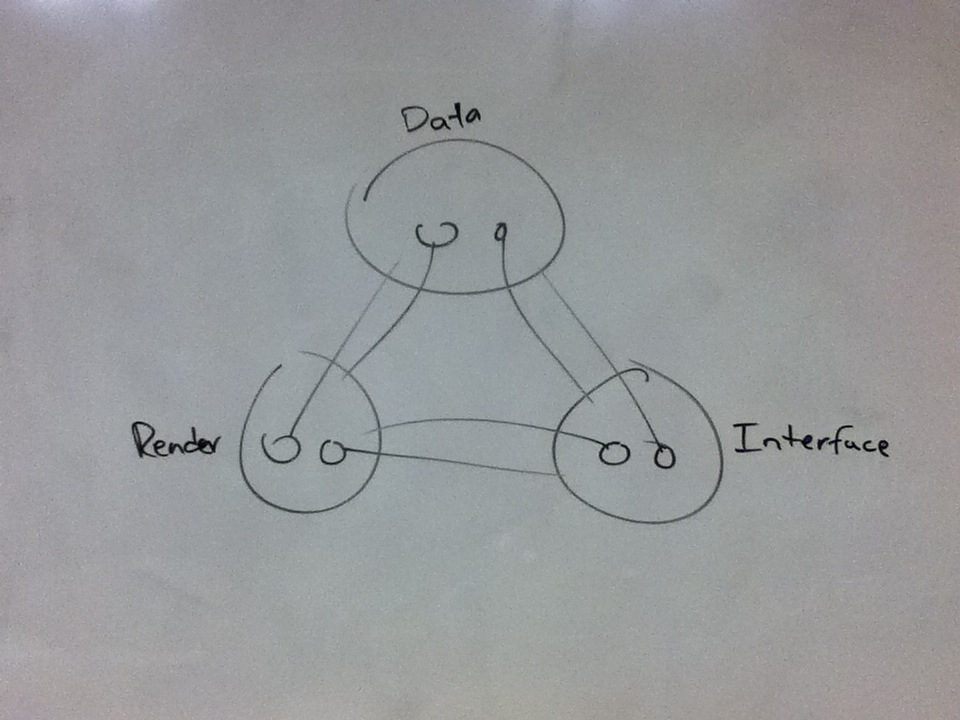
\includegraphics[width=1\textwidth]{./whiteboards/portion-checks}
\end{center}

\end{document}
